% 3D Cone
% Author: Gene Ressler. Adapted to TikZ by Kjell Magne Fauske.
% See http://www.frontiernet.net/~eugene.ressler/ for more details.
\documentclass{article}
\usepackage{tikz}
\usepackage{verbatim}

\begin{comment}
:Title: 3D cone
:Tags: 3D, Transparency

An annotated three dimensional drawing with transparency effects. The code has been
generated using Sketch_. Sketch is a small, simple system for producing line drawings 
of two- or three-dimensional solid objects and scenes. Sketch accepts a tiny scene 
description language and generates PGF/TikZ or PSTricks code. 
Sketch also supports hidden surface removal and its easy to embed TikZ and LaTeX code 
in your drawings.

The Sketch code used to generate the drawing is available for download_. 
A detailed description_ of the code can be found in the Sketch manual_.

**Update:** Read more about Sketch in my notebook entry: `An introduction to Sketch 3D 
for PGF and TikZ users`__. 

.. __: http://www.fauskes.net/nb/introduction-to-sketch/

:Author: Gene Ressler. Adapted to TikZ by Kjell Magne Fauske.

.. _Sketch: http://www.frontiernet.net/~eugene.ressler/
.. _description: http://www.frontiernet.net/~eugene.ressler/manual.html#A-technical-drawing
.. _manual: http://www.frontiernet.net/~eugene.ressler/manual.html
.. _download: http://www.fauskes.net/media/pgftikzexamples/data/cone.sk
\end{comment}


\begin{document}
\pagestyle{empty}

% The following code is generated by Sketch. I have edited it a bit
% to make it easier to read.
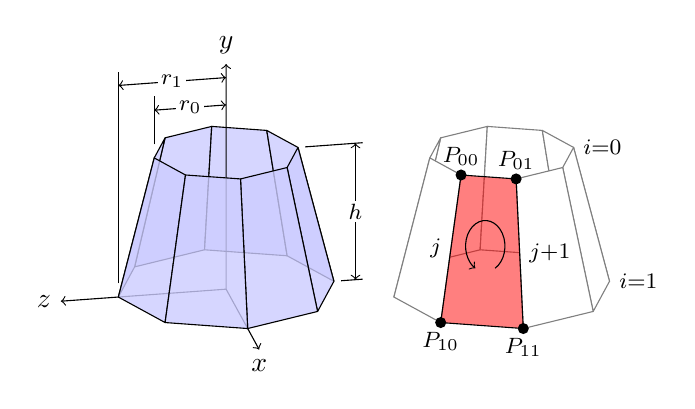
\begin{tikzpicture}[join=round]
    \tikzstyle{conefill} = [fill=blue!20,fill opacity=0.8]
    \tikzstyle{ann} = [fill=white,font=\footnotesize,inner sep=1pt]
    \tikzstyle{ghostfill} = [fill=white]
         \tikzstyle{ghostdraw} = [draw=black!50]
    \filldraw[conefill](-.775,1.922)--(-1.162,.283)--(-.274,.5)
                        --(-.183,2.067)--cycle;
    \filldraw[conefill](-.183,2.067)--(-.274,.5)--(.775,.424)
                        --(.516,2.016)--cycle;
    \filldraw[conefill](.516,2.016)--(.775,.424)--(1.369,.1)
                        --(.913,1.8)--cycle;
    \filldraw[conefill](-.913,1.667)--(-1.369,-.1)--(-1.162,.283)
                        --(-.775,1.922)--cycle;
    \draw(1.461,.107)--(1.734,.127);
    \draw[arrows=<->](1.643,1.853)--(1.643,.12);
    \filldraw[conefill](.913,1.8)--(1.369,.1)--(1.162,-.283)
                        --(.775,1.545)--cycle;
    \draw[arrows=->,line width=.4pt](.274,-.5)--(0,0)--(0,2.86);
    \draw[arrows=-,line width=.4pt](0,0)--(-1.369,-.1);
    \draw[arrows=->,line width=.4pt](-1.369,-.1)--(-2.1,-.153);
    \filldraw[conefill](-.516,1.45)--(-.775,-.424)--(-1.369,-.1)
                        --(-.913,1.667)--cycle;
    \draw(-1.369,.073)--(-1.369,2.76);
    \draw(1.004,1.807)--(1.734,1.86);
    \filldraw[conefill](.775,1.545)--(1.162,-.283)--(.274,-.5)
                        --(.183,1.4)--cycle;
    \draw[arrows=<->](0,2.34)--(-.913,2.273);
    \draw(-.913,1.84)--(-.913,2.447);
    \draw[arrows=<->](0,2.687)--(-1.369,2.587);
    \filldraw[conefill](.183,1.4)--(.274,-.5)--(-.775,-.424)
                        --(-.516,1.45)--cycle;
    \draw[arrows=<-,line width=.4pt](.42,-.767)--(.274,-.5);
    \node[ann] at (-.456,2.307) {$r_0$};
    \node[ann] at (-.685,2.637) {$r_1$};
    \node[ann] at (1.643,.987) {$h$};
    \path (.42,-.767) node[below] {$x$}
        (0,2.86) node[above] {$y$}
        (-2.1,-.153) node[left] {$z$};
    % Second version of the cone
    \begin{scope}[xshift=3.5cm]
    \filldraw[ghostdraw,ghostfill](-.775,1.922)--(-1.162,.283)--(-.274,.5)
                                   --(-.183,2.067)--cycle;
    \filldraw[ghostdraw,ghostfill](-.183,2.067)--(-.274,.5)--(.775,.424) 
                                   --(.516,2.016)--cycle;
    \filldraw[ghostdraw,ghostfill](.516,2.016)--(.775,.424)--(1.369,.1)
                                   --(.913,1.8)--cycle;
    \filldraw[ghostdraw,ghostfill](-.913,1.667)--(-1.369,-.1)--(-1.162,.283)
                                   --(-.775,1.922)--cycle;
    \filldraw[ghostdraw,ghostfill](.913,1.8)--(1.369,.1)--(1.162,-.283)
                                   --(.775,1.545)--cycle;
    \filldraw[ghostdraw,ghostfill](-.516,1.45)--(-.775,-.424)--(-1.369,-.1)
                                   --(-.913,1.667)--cycle;
    \filldraw[ghostdraw,ghostfill](.775,1.545)--(1.162,-.283)--(.274,-.5)
                                   --(.183,1.4)--cycle;
    \filldraw[fill=red,fill opacity=0.5](-.516,1.45)--(-.775,-.424)--(.274,-.5)
                                         --(.183,1.4)--cycle;
    \fill(-.775,-.424) circle (2pt);
    \fill(.274,-.5) circle (2pt);
    \fill(-.516,1.45) circle (2pt);
    \fill(.183,1.4) circle (2pt);
    \path[font=\footnotesize]
            (.913,1.8) node[right] {$i\hbox{$=$}0$}
            (1.369,.1) node[right] {$i\hbox{$=$}1$};
    \path[font=\footnotesize]
            (-.645,.513) node[left] {$j$}
            (.228,.45) node[right] {$j\hbox{$+$}1$};
    \draw (-.209,.482)+(-60:.25) [yscale=1.3,->] arc(-60:240:.25);
    \fill[black,font=\footnotesize]
                    (-.516,1.45) node [above] {$P_{00}$}
                    (-.775,-.424) node [below] {$P_{10}$}
                    (.183,1.4) node [above] {$P_{01}$}
                    (.274,-.5) node [below] {$P_{11}$};
    \end{scope}
\end{tikzpicture}

\end{document}

